%%%%(c) COPYRIGHT NOTICE%FOLDUP
%%%%(c)
%%%%(c)  This file is a portion of the source for the textbook
%%%%(c)
%%%%(c)    Numerical Methods Course Notes,
%%%%(c)    Copyright 2004-2010 by Steven E. Pav
%%%%(c)
%%%%(c)  See the file COPYING.txt for copying conditions
%%%%(c)
%%%%(c)%UNFOLD

%%throat clearing%FOLDUP
\typeout{-- interpolate.tex}
\typeout{-- N� 2004-2010 Steven E. Pav}
%UNFOLD

%%local commands%FOLDUP
%UNFOLD

\chapter{Interpolation}

%%%%%%%%%%%%%%%%%%%%%%%%%%%%%%%%%%%%%%%%%%%%%%%
\section{Polynomial Interpolation}%FOLDUP
\label{sec:polyInt}

We consider the problem of finding a polynomial that interpolates a given set
of values:
\[
\begin{array}{c||c|c|c|c}
x & x_0 & x_1 & \ldots & x_n\\
\hline
y & y_0 & y_1 & \ldots & y_n\\
\end{array}
\]
where the $x_i$ are all distinct.  A polynomial $p(x)$ is said to interpolate
these data if $p(x_i) = y_i$ for $i=0,1,\ldots,n.$  The $x_i$ values are called
``nodes.''

Sometimes, we will consider a variant of this problem: we have some black box
function, $f(x),$ which we want to approximate with a polynomial $p(x).$  We do
this by finding the polynomial interpolant to the data
\[
\begin{array}{c||c|c|c|c}
x & x_0 & x_1 & \ldots & x_n\\
\hline
f(x) & f(x_0) & f(x_1) & \ldots & f(x_n)\\
\end{array}
\]
for some choice of distinct nodes $x_i$.

%%%%%%%%%%%%%%%%%%%%%%%%%%%%%%%%%%%%%%%%%%%%%%%
\subsection{Lagranges Method}%FOLDUP

As you might have guessed, for any such set of data, there is an $n$-degree
polynomial that interpolates it.  We present a constructive proof of this fact
by use of Lagrange Polynomials.  

\begin{bkdefinition}[Lagrange Polynomials]%FOLDUP
For a given set of $n+1$ nodes $x_i,$ the Lagrange polynomials are the $n+1$
polynomials $\ell_i$ defined by
\[
\ell_i(x_j) = \delta_{ij} = \left\{\begin{array}{rl}0 & \text{if } i\ne j\\1 &
\text{if } i=j\end{array} \right.
\]
\index{Lagrange Polynomials}
\end{bkdefinition}
%UNFOLD

Then we define the interpolating polynomial as 
\[p_n(x) = \sum_{i=0}^n y_i \ell_i(x).\]

If each Lagrange Polynomial is of degree at most $n,$ then $p_n$ also has this
property.  The Lagrange Polynomials can be characterized as follows:
\begin{empheq}[innerbox=\widefbox]{equation}
\ell_i(x) = \prod_{j=0,\,j\ne i}^{n} \frac{x - x_j}{x_i - x_j}.
\label{eqn:lagpolydef}
\end{empheq}
By evaluating this product for each $x_j,$ we see that this is indeed a
characterization of the Lagrange Polynomials.  Moreover, each polynomial is
clearly the product of $n$ monomials, and thus has degree no greater than $n.$

This gives the theorem

\begin{bktheorem}[Interpolant Existence and Uniqueness]\label{thm:polyint}%FOLDUP
Let \setBIdx{x_i}{i=0}{n} be distinct nodes.  Then for any values at the nodes,
\setBIdx{y_i}{i=0}{n}, there is exactly one polynomial, $p(x)$ of degree no
greater than $n$ such that $p(x_i) = y_i$ for $i=\zerotox{n}.$
\end{bktheorem}
\begin{proof}
The Lagrange Polynomial construction gives existence of such a polynomial
$p(x)$ of degree no greater than $n.$  

Suppose there were two such polynomials,
call them $p(x),q(x),$ each of degree no greater than
$n,$ both interpolating the data.  Let $r(x) = p(x) - q(x).$  Note that
$r(x)$ can have degree no greater than $n,$ yet it has roots at
$x_0,x_1,\ldots,x_n.$  The only polynomial of degree $\le n$ that has $n+1$
distinct roots is the zero polynomial, \ie $0 \equiv r(x) = p(x) - q(x).$
Thus $p(x),q(x)$ are equal everywhere, \ie they are the same polynomial.
\end{proof}
%UNFOLD
\begin{bkexprob}%FOLDUP
Construct the polynomial interpolating the data
\[
\begin{array}{c||c|c|c}
x & 1 & \half & 3\\
\hline
y & 3 & -10 & 2\\
\end{array}
\]
by using Lagrange Polynomials.
\begin{bksolution}
We construct the Lagrange Polynomials:
\begin{align*}
\ell_0(x) &= \frac{(x-\half)(x-3)}{(1-\half)(1-3)} = -(x-\half)(x-3)\\
\ell_1(x) &= \frac{(x-1)(x-3)}{(\half - 1)(\half-3)} = \frac{4}{5} (x-1)(x-3)\\
\ell_2(x) &= \frac{(x-1)(x-\half)}{(3 - 1)(3-\half)} = \frac{1}{5} (x-1)(x-\half)
\end{align*}
Then the interpolating polynomial, in ``Lagrange Form'' is
\[
p_2(x) = -3 (x-\half)(x-3) - 8 (x-1)(x-3) + \frac{2}{5} (x-1)(x-\half)
\]
\end{bksolution}
\end{bkexprob}%UNFOLD

\begin{figure}[htb]%FOLDUP
\begin{center}
\includegraphics[height=0.7\columnwidth, angle=270,angle=0,clip=]{lagrange.eps}
\end{center}
\caption{The 3 Lagrange polynomials for the example are shown. Verify,
graphically, that these polynomials have the property $\ell_i(x_j) =
\delta_{ij}$ for the nodes $1,\half,3$.}\label{fig:lagrange}
\end{figure}%UNFOLD
\begin{figure}[htb]%FOLDUP
\begin{center}
\includegraphics[height=0.6\columnwidth, angle=270,angle=0,clip=]{lpoly.eps}
\end{center}
\caption{The interpolating polynomial for the example is
shown.}\label{fig:lpoly}
\end{figure}%UNFOLD
%UNFOLD
%%%%%%%%%%%%%%%%%%%%%%%%%%%%%%%%%%%%%%%%%%%%%%%
\subsection{Newton's Method}%FOLDUP

There is another way to prove existence.  This method is also constructive, and
leads to a different algorithm for constructing the interpolant.  One way to
view this construction is to imagine how one would update the Lagrangian form
of an interpolant.  That is, suppose some data were given, and the
interpolating polynomial calculated using Lagrange Polynomials;  then a new
point was given \tuple{x_{n+1},y_{n+1}}, and an interpolant for the augmented
set of data is to be found.  Each Lagrange Polynomial would have to be updated.
This could take a lot of calculation (especially if $n$ is large).  

So the alternative method constructs the polynomials iteratively.  Thus we
create polynomials $p_k(x)$ such that $p_k(x_i) = y_i$ for $0\le i \le k.$
This is simple for $k=0,$ we simply let
\[
p_0(x) = y_0,
\]
the constant polynomial with value $y_0.$  Then assume we have a proper
$p_k(x)$ and want to construct $p_{k+1}(x).$  The following construction works:
\[
p_{k+1}(x) = p_k(x) + c (x-x_0)(x-x_1)\cdots(x-x_k),
\]
for some constant $c.$  Note that the second term will be zero for any $x_i$
for $0\le i \le k,$ so $p_{k+1}(x)$ will interpolate the data at
$x_0,x_1,\ldots,x_k.$  To get the value of the constant we calculate $c$ such
that
\[
y_{k+1} = p_{k+1}(x_{k+1}) = p_k(x_{k+1}) + c
(x_{k+1}-x_0)(x_{k+1}-x_1)\cdots(x_{k+1}-x_k).
\]

This construction is known as Newton's Algorithm, and the resultant form is
Newton's form of the interpolant

\begin{bkexprob}\label{bkexp:interpagain}%FOLDUP
Construct the polynomial interpolating the data
\[
\begin{array}{c||c|c|c}
x & 1 & \half & 3\\
\hline
y & 3 & -10 & 2\\
\end{array}
\]
by using Newton's Algorithm.
\begin{bksolution}
We construct the polynomial iteratively:
\begin{align*}
p_0(x) &= 3\\
p_1(x) &= 3 + c (x-1)
\end{align*}
We want $-10 = p_1(\half) = 3 + c (-\half),$ and thus $c = 26.$  Then
\[
p_2(x) = 3 + 26 (x-1) + c (x-1)(x-\half)
\]
We want $2 = p_2(3) = 3 + 26 (2) + c (2)(\frac{5}{2}),$ and thus $c =
\frac{-53}{5}.$  Then we get
\[
p_2(x) = 3 + 26 (x-1) + \frac{-53}{5} (x-1)(x-\half).
\]
\end{bksolution}
\end{bkexprob}%UNFOLD

Does Newton's Algorithm give a different polynomial?  It is
easy to show, by induction, that the degree of $p_n(x)$ is no greater than $n.$
Then, by \thmref{polyint}, it must be the same polynomial as the Lagrange
interpolant.

The two methods give the same interpolant, we may wonder ``Which should we
use?''  Newton's Algorithm seems more flexible--it can deal with
adding new data.  There also happens to be a way of storing Newton's form of
the interpolant that makes the polynomial simple to evaluate (in the sense of
number of calculations required).

%UNFOLD
%%%%%%%%%%%%%%%%%%%%%%%%%%%%%%%%%%%%%%%%%%%%%%%
\subsection{Newton's Nested Form} %FOLDUP

Recall the iterative construction of Newton's Form:
\[p_{k+1}(x) = p_k(x) + c_k (x-x_0)(x-x_1)\cdots(x-x_k).\]
The previous iterate $p_k(x)$ was constructed similarly, so we 
can write:
\[p_{k+1}(x) = \Bracks{p_{k-1}(x) + c_{k-1} (x-x_0)(x-x_1)\cdots(x-x_{k-1})} + c_k (x-x_0)(x-x_1)\cdots(x-x_k).\]
Continuing in this way we see that we can write
\begin{empheq}[innerbox=\widefbox]{equation}
p_n(x) = \sum_{k=0}^{n} c_k \Bracks{\prod_{0 \le j < k} (x-x_j)},
\label{eqn:newtongathered}
\end{empheq}
where an empty product has value $1$ by convention.
This can be rewritten in a funny form, where a monomial is factored out of each
successive summand:
\[p_n(x) = c_0 + (x-x_0) \wrapbracks{c_1 + (x-x_1)\wrapbracks{c_2 +
(x-x_2)\Bracks{\ldots}}}\]

Supposing for an instant that the constants $c_k$ were known, this provides a
better way of calculating $p_n(t)$ at arbitrary $t.$  By ``better'' we mean
requiring few multiplications and additions.  This nested calculation is
performed iteratively:

\begin{align*}
v_0 &= c_n\\
v_1 &= c_{n-1} + (t-x_{n-1}) v_0\\
v_2 &= c_{n-2} + (t-x_{n-2}) v_1\\
&\vdots&\\
v_n &= c_0 + (t-x_0) v_{n-1}
\end{align*}

This requires only $n$ multiplications and $2n$ additions.  Compare this with
the number required for using the Lagrange form: at least $n^2$ additions and
multiplications.

%UNFOLD
%%%%%%%%%%%%%%%%%%%%%%%%%%%%%%%%%%%%%%%%%%%%%%%
\subsection{Divided Differences} %FOLDUP

It turns out that the coefficients $c_k$ for Newton's nested form can be
calculated relatively easily by using \emph{divided differences}.  We assume,
for the remainder of this section, that we are considering interpolating a
function, that is, we have values of $f(x_i)$ at the nodes $x_i.$  

\begin{bkdefinition}[Divided Differences]
For a given collection of nodes \setBIdx{x_i}{i=0}{n} and values
\setBIdx{f(x_i)}{x=0}{n}, a \kth{k} order divided difference is a function of
$k+1$ (not necessarily distinct) nodes, written as 
\[
f\Bracks{x_{i_0},x_{i_1},\ldots,x_{i_k}}
\]
The divided differences are defined recursively as follows:
\begin{compactitem}
\item The \kth{0} order divided differences are simply defined:
\[f\Bracks{x_i} = f(x_i).\]
\item Higher order divided differences are the ratio of differences:
\[
f\Bracks{x_{i_0},x_{i_1},\ldots,x_{i_k}} =
\frac{ f\Bracks{x_{i_1},x_{i_2},\ldots,x_{i_k}} -
 f\Bracks{x_{i_0},x_{i_1},\ldots,x_{i_{k-1}}} }{x_{i_k} - x_{i_0}}
\]
\end{compactitem}
\index{divided differences}
\end{bkdefinition}

We care about divided differences because coefficients for the Newton nested
form are divided differences: 
\begin{empheq}[innerbox=\widefbox]{equation}
c_k = f\Bracks{x_0,x_1,\ldots,x_k}.
\label{eqn:newtoncoeffs}
\end{empheq}
Because we are only interested in the Newton method coefficients, we will
only consider divided differences with successive nodes, \ie those of the form 
$f\Bracks{x_j,x_{j+1},\ldots,x_{j+k}}$.  In this case the higher order
differences can more simply be written as 
\[
f\Bracks{x_{j},x_{j+1},\ldots,x_{j+k}} =
\frac{ f\Bracks{x_{j+1},x_{j+2},\ldots,x_{j+k}} -
 f\Bracks{x_{j},x_{j+1},\ldots,x_{j+{k-1}}} }{x_{j+k} - x_{j}}
\]

The graphical way to calculate these things is a ``pyramid
scheme''\footnote{That's supposed to be a joke.}, where you compute the
following table columnwise, from left to right:
\[
\begin{array}{c||c|c|c|c}
x & f[\,] & f[\,,\,] & f[\,,\,,\,] & f[\,,\,,\,,\,]\\
\hline
x_0 & f[x_0] & & &\\
 & & f[x_0,x_1] & &\\
x_1 & f[x_1] & & f[x_0,x_1,x_2] &\\
 & & f[x_1,x_2] & & f[x_0,x_1,x_2,x_3]\\
x_2 & f[x_2] & & f[x_1,x_2,x_3] &\\
 & & f[x_2,x_2] & &\\
x_3 & f[x_3] & & &\\
\end{array}
\]
Note that by definition, the first column just echoes the data: $f[x_i] =
f(x_i).$

We drag out our example one last time:

\begin{bkexprob}%FOLDUP
Find the divided differences for the following data
\[
\begin{array}{c||c|c|c}
x & 1 & \half & 3\\
\hline
f(x) & 3 & -10 & 2\\
\end{array}
\]
\begin{bksolution}
We start by writing in the data:
\[
\begin{array}{c||c|c|c}
x & f[\,] & f[\,,\,] & f[\,,\,,\,] \\
\hline
1 & 3 & & \\
 & &  & \\
\half & -10 & &  \\
 & & & \\
3 & 2 & & \\
\end{array}
\]
Then we calculate:
\[
f[x_0,x_1] = \frac{-10 - 3}{\haLf - 1} = 26, \quad\text{and}\quad
f[x_1,x_2] = \frac{2 - -10}{3 - \haLf} = 24/5.
\]
Adding these to the table, we have
\[
\begin{array}{c||c|c|c}
x & f[\,] & f[\,,\,] & f[\,,\,,\,] \\
\hline
1 & 3 & & \\
 & & 26  & \\
\half & -10 & & \\
 & & \frac{24}{5} & \\
3 & 2 & & \\
\end{array}
\]
Then we calculate
\[
f[x_0,x_1,x_2] = \frac{24/5 - 26}{3 - 1} = \frac{-53}{5}.
\]
So we complete the table:
\[
\begin{array}{c||c|c|c}
x & f[\,] & f[\,,\,] & f[\,,\,,\,] \\
\hline
1 & 3 & & \\
 & & 26  & \\
\half & -10 & & \frac{-53}{5} \\
 & & \frac{24}{5} & \\
3 & 2 & & \\
\end{array}
\]
You should verify that along the top line of this pyramid you can read off the
coefficients for Newton's form, as found in \bkexpref{interpagain}.
\end{bksolution}
\end{bkexprob}%UNFOLD
%UNFOLD
%UNFOLD
%%%%%%%%%%%%%%%%%%%%%%%%%%%%%%%%%%%%%%%%%%%%%%%
\section{Errors in Polynomial Interpolation}%FOLDUP
\label{sec:polyerror}
\depson{sec:polyInt}{sec:polyerror}

%intro%FOLDUP
%\figref{badrunge}%%%%%%%%%%%%%%%%%%FOLDUP
\begin{figure}[htbp!]
\begin{center}
%\subfigure[3,7,10 equally spaced nodes]{
\subfloat[3,7,10 equally spaced nodes]{
	\label{fig:rsmall}
	\includegraphics[height=0.85\columnwidth, angle=270,clip=]{rungesmall.ps}}\\
%\subfigure[15 equally spaced nodes]{
\subfloat[15 equally spaced nodes]{
	\label{fig:rfif}
	\includegraphics[height=0.47\columnwidth, angle=270,clip=]{runge15.ps}}
%\subfigure[50 equally spaced nodes]{
\subfloat[50 equally spaced nodes]{
	\label{fig:rfifty}
	\includegraphics[height=0.47\columnwidth, angle=270,clip=]{runge50.ps}}
\end{center}
\caption{The Runge function is poorly interpolated at $n$ equally spaced nodes,
as $n$ gets large.  At first, the interpolations appear to improve with larger
$n$, as in (a).  In (b) it becomes apparent that the interpolant is good in
center of the interval, but bad at the edges.  As shown in (c), this gets worse
as $n$ gets larger.}\label{fig:badrunge}
\end{figure}
%UNFOLD
We now consider two questions: 
\begin{compactenum}
\item If we want to interpolate some function $f(x)$ at $n+1$ nodes over some
closed interval, how should we pick the nodes?
\item How accurate can we make a polynomial interpolant over a closed interval?
\end{compactenum}

You may be surprised to find that the answer to the first question is
\emph{not} that we should make the $x_i$ equally spaced over the closed
interval, as the following example illustrates.

\begin{bkexample}[Runge Function]\label{bkex:rungef}%FOLDUP
Let 
\[f(x) = \Parens{1+x^2}^{-1},\]
(known as the \emph{Runge Function}), and let $p_n(x)$ interpolate $f$ on $n$
equally spaced nodes, including the endpoints, on \ccinv{-5}{5}. Then
\[\lim_{n\to\infty} \max_{x\in\ccinv{-5}{5}} \abs{p_n(x) - f(x)} = \infty.\]
\index{Runge Function}
This behaviour is shown in \figref{badrunge}.
\end{bkexample}
%UNFOLD

It turns out that a much better choice is related to the
\emph{Chebyshev Polynomials} (``of the first kind'').  If our closed interval
is \ccinv{-1}{1}, then we want to define our nodes as 
\[
x_i = \cos\Bracks{\Parens{\frac{2i+1}{2n+2}} \pi},\quad0\le i\le n.
\]
\index{Chebyshev Polynomials}
%Note that this is different than what appears in your book.  This book is in
%error.  If you do not trust me, look at the fifth edition, or look at 
%equation (9) of%
%\begin{verbatim}http://mathworld.wolfram.com/ChebyshevPolynomialoftheFirstKind.html\end{verbatim}%

Literally interpreted, these \emph{Chebyshev Nodes} are the projections of
points uniformly spaced on a semi circle;  see \figref{chebynodes}.
By using the Chebyshev nodes, a good polynomial interpolant of the Runge
function of \bkexref{rungef} can be found, as shown in \figref{rungecheb}.

%\figref{chebynodes}%%%%%%%%%%%%%%%%FOLDUP
\begin{figure}[htb!]
\begin{center}
\psfrag{1}{$1$}
\psfrag{hyphen }{$-$}
\includegraphics[height=0.7\columnwidth, angle=270,clip=]{chebynodes.eps}
\end{center}
\caption{The Chebyshev nodes are the projections of nodes equally spaced on a
semi circle.}\label{fig:chebynodes}
\end{figure}
%UNFOLD
%\figref{rungecheb}%%%%%%%%%%%%%%%%%%FOLDUP
\begin{figure}[htb!]
\begin{center}
%\subfigure[3,7,10 Chebyshev nodes]{
\subfloat[3,7,10 Chebyshev nodes]{
	\label{fig:rchsm}
	\includegraphics[height=0.47\columnwidth, angle=270,clip=]{rungechebsm.ps}}
%\subfigure[17 Chebyshev nodes]{
\subfloat[17 Chebyshev nodes]{
	\label{fig:rchsev}
	\includegraphics[height=0.47\columnwidth, angle=270,clip=]{rungecheb17.ps}}
\end{center}
\caption{The Chebyshev nodes yield good polynomial interpolants of the
Runge function.  Compare these figures to those of \figref{badrunge}.  For more
than about 25 nodes, the interpolant is indistinguishable from the Runge
function by eye.}\label{fig:rungecheb}
\end{figure}
%UNFOLD
%UNFOLD
%%%%%%%%%%%%%%%%%%%%%%%%%%%%%%%%%%%%%%%%%%%%%%%
\subsection{Interpolation Error Theorem}%FOLDUP

We did not just invent the Chebyshev nodes.  The fact that they are ``good''
for interpolation follows from the following theorem:

\begin{bktheorem}[Interpolation Error Theorem]\label{thm:interror}%FOLDUP
Let $p$ be the polynomial of degree at most $n$ interpolating function $f$ at
the $n+1$ distinct nodes $x_0,x_1,\ldots,x_n$ on \ccinv{a}{b}.  Let $f^{(n+1)}$
be continuous.  Then for each $x \in \ccinv{a}{b}$ there is some
$\xi\in\ccinv{a}{b}$ such that
\[
f(x) - p(x) = \oneby{\Parens{n+1}!} f^{(n+1)}(\xi) \prod_{i=0}^n \Parens{x-x_i}.
\]
\end{bktheorem}
%UNFOLD
You should be thinking that the term on the right hand side resembles the error
term in Taylor's Theorem.  
\begin{proof}%FOLDUP
First consider when $x$ is one of the nodes $x_i$; in this case both the LHS
and RHS are zero.  So assume $x$ is not a node.  Make the following definitions
\begin{align*}
w(t) &= \prod_{i=0}^n \Parens{t-x_i},\\
c &= \frac{f(x) - p(x)}{w(x)},\\
\phi(t) &= f(t) - p(t) - cw(t).
\end{align*}
Since $x$ is not a node, $w(x)$ is nonzero.  Now note that $\phi(x_i)$ is zero
for each node $x_i,$ and that by definition of $c,$ that $\phi(x) = 0$ for our
$x.$  That is $\phi(t)$ has $n+2$ roots.

Some other facts: $f,p,w$ have $n+1$ continuous derivatives, by assumption and
definition; thus $\phi$ has this many continuous derivatives.  Apply Rolle's
Theorem to $\phi(t)$ to find that $\phi'(t)$ has $n+1$ roots.  Then apply
Rolle's Theorem again to find $\phi''(t)$ has $n$ roots.  In this way we see
that $\phi^{(n+1)}(t)$ has a root, call it $\xi.$  That is
\[0 = \phi^{(n+1)}(\xi) = f^{(n+1)}(\xi) - p^{(n+1)}(\xi) - c w^{(n+1)}(\xi).\]

But $p(t)$ is a polynomial of degree $\le n,$ so $p^{(n+1)}$ is identically
zero.  And $w(t)$ is a polynomial of degree $n+1$ in $t$, so its \kth{n+1}
derivative is easily seen to be $(n+1)!$  Thus
\begin{align*}
0 &= f^{(n+1)}(\xi) - c (n+1)!\\
c (n+1)! &= f^{(n+1)}(\xi)\\
\frac{f(x) - p(x)}{w(x)} &= \oneby{(n+1)!} f^{(n+1)}(\xi)\\
f(x) - p(x) &= \oneby{(n+1)!} f^{(n+1)}(\xi) w(x),
\end{align*}
which is what was to be proven.
\end{proof}
%UNFOLD

Thus the error in a polynomial interpolation is given as 
\[
f(x) - p(x) = \oneby{\Parens{n+1}!} f^{(n+1)}(\xi) \prod_{i=0}^n \Parens{x-x_i}.
\]
We have no control over the function $f(x)$ or its derivatives, and once the
nodes and $f$ are fixed, $p$ is determined; thus the only way we can make the error
$\abs{f(x) - p(x)}$ small is by judicious choice of the nodes $x_i.$

The Chebyshev nodes on \ccinv{-1}{1} have the remarkable property that 
\[\abs{\prod_{i=0}^n \Parens{t-x_i}} \le 2^{-n}\]
for any $t \in \ccinv{-1}{1}.$  Moreover, it can be shown that for \emph{any}
choice of nodes $x_i$ that
\[\max_{t\in\ccinv{-1}{1}} \abs{\prod_{i=0}^n \Parens{t-x_i}} \ge 2^{-n}.\]
Thus the Chebyshev nodes are considered the best for polynomial
interpolation.

Merging this result with \thmref{interror}, the error for polynomial
interpolants defined on Chebyshev nodes can be bounded as 
\[
\abs{f(x) - p(x)} \le \oneby{2^n\Parens{n+1}!} 
	\max\limits_{\xi \in \ccinv{-1}{1}} \abs{f^{(n+1)}(\xi)}.
\]

The Chebyshev nodes can be rescaled and shifted for use on the general interval
\ccinv{\alpha}{\beta}.  In this case they take the form
\[
x_i = \frac{\beta - \alpha}{2} \cos\Bracks{\Parens{\frac{2i+1}{2n+2}} \pi} +
\frac{\alpha+\beta}{2},\quad0\le i\le n.
\]
In this case, the rescaling of the nodes changes the bound on $\prod
\wrapparens{t - x_i}$
so the overall error bound becomes
\[
\abs{f(x) - p(x)} \le \frac{\Parens{\beta-\alpha}^{n+1}}{2^{2n+1}\Parens{n+1}!} 
	\max\limits_{\xi \in \ccinv{\alpha}{\beta}} \abs{f^{(n+1)}(\xi)},
\]
for $x \in \ccinv{\alpha}{\beta}.$

\begin{bkexprob}\label{bkexp:howmanycheby}%FOLDUP
How many Chebyshev nodes are required to interpolate the function
$f(x) = \sin(x) + \cos(x)$ to within $10^{-8}$ on the interval \ccinv{0}{\pi}?
\begin{bksolution}
We first find the derivatives of $f$
\begin{align*}
f'(x) &= \cos(x) - \sin(x)\\
f''(x) &= -\sin(x) - \cos(x)\\
f'''(x) &= -\cos(x) + \sin(x)\\
&\vdots 
\end{align*}

As a crude approximation we can assert that
\[\abs{f^{(k)}(x)} \le \abs{\cos{x}} + \abs{\sin{x}} \le 2.\]
Thus it suffices to take $n$ large enough such that
\[
\frac{\pi^{n+1}}{2^{2n+1}\Parens{n+1}!} 2 \le 10^{-8}
\]
By trial and error we see that $n=10$ suffices.
\end{bksolution}
\end{bkexprob}%UNFOLD

%UNFOLD
%%%%%%%%%%%%%%%%%%%%%%%%%%%%%%%%%%%%%%%%%%%%%%%
\subsection{Interpolation Error for Equally Spaced Nodes}%FOLDUP

Despite the proven superiority of Chebyshev Nodes, and the problems with the
Runge Function, equally spaced nodes are frequently used for interpolation,
since they are easy to calculate\footnote{Never underestimate the power of
laziness.}.  We now consider
bounding
\[\max_{x \in \ccinv{a}{b}} \prod_{i=0}^{n} \abs{x-x_i},\]
where
\[x_i = a + hi = a + \frac{(b-a)}{n}i,\qquad i=0,1,\ldots,n.\]

Start by picking an $x.$  We can assume $x$ is not one of the nodes, otherwise
the product in question is zero.  Then $x$ is between some $x_j,x_{j+1}$  We
can show that
\[\abs{x-x_j}\abs{x-x_{j+1}} \le \frac{h^2}{4}.\]
by simple calculus.

Now we claim that $\abs{x-x_i} \le \Parens{j-i+1}h$ for $i<j,$ and 
$\abs{x-x_i} \le \Parens{i-j}h$ for $j+1<i.$
Then
\[\prod_{i=0}^{n} \abs{x-x_i} \le
\frac{h^2}{4}\Bracks{\Parens{j+1}!h^{j}}\Bracks{\Parens{n-j}!h^{n-j-1}}.\]
It can be shown that $(j+1)!(n-j)! \le n!,$ and so we get an overall bound
\[\prod_{i=0}^{n} \abs{x-x_i} \le \frac{h^{n+1} n!}{4}.\]

The interpolation theorem then gives us
\[
\abs{f(x) - p(x)} \le \frac{h^{n+1}}{4\Parens{n+1}} 
	\max\limits_{\xi \in \ccinv{a}{b}} \abs{f^{(n+1)}(\xi)},
\]
where $h = (b-a) / n.$

The reason this result does not seem to apply to Runge's Function is that $f^{(n)}$
for Runge's Function becomes unbounded as $n\to\infty.$

\begin{bkexprob}%FOLDUP
How many equally spaced nodes are required to interpolate the function
$f(x) = \sin(x) + \cos(x)$ to within $10^{-8}$ on the interval \ccinv{0}{\pi}?
\begin{bksolution}
As in \bkexpref{howmanycheby}, we make the crude approximation
\[\abs{f^{(k)}(x)} \le \abs{\cos{x}} + \abs{\sin{x}} \le 2.\]

Thus we want to make $n$ sufficiently large such that
\[\frac{h^{n+1}}{4(n+1)} 2 \le 10^{-8},\]
where $h = (\pi - 0) / n$.  That is we want to find $n$ large enough such that
\[\frac{\pi^{n+1}}{2n^{n+1}(n+1)} \le 10^{-8},\]
By simply trying small numbers, we can see this is satisfied if $n=12.$
\end{bksolution}
\end{bkexprob}%UNFOLD

%UNFOLD
%%%%%%%%%%%%%%%%%%%%%%%%%%%%%%%%%%%%%%%%%%%%%%%
%\subsection{Interpolating Black Box Functions}%FOLDUP
%
%Many of the techniques we have looked at for interpolation have relied on
%some pretty broad assumptions about the function $f(x)$: we have assumed
%continuity and boundedness of derivatives.   You may wonder if there is any way
%to \emph{check}, algorithmically, if some arbitrary black box function satisfies 
%these properties.
%
%The sad fact is that there is \emph{no} way of testing existence of derivatives
%of a black box function $f(x),$ or of the continuity or boundedness of those derivatives.
%Here's why:
%
%Imagine some subroutine that took a black box function $f(x),$ tested it's
%value at a finite number of values, say ${x}_0,{x}_1,\ldots,{x}_n,$
%then declares that $f(x)$ has $k$ continuous derivatives, and it's \kth{k}
%derivative is bounded by some constant $M_k$.  
%
%However, there is some function $g(x)$ which happens to interpolate
%$f(x)$ at ${x}_0,{x}_1,\ldots,{x}_n,$ and which is not continuous,
%and thus has no derivatives.  To construct $g(x),$ let $p(x)$ be the unique
%polynomial of degree $\le n$ that interpolates $f(x)$ at these nodes.  Then let
%\[
%g(x) = \left\{ \begin{array}{cl} p(x) & \text{if $x$ is a node $x_i,$ or $x$
%is rational}\\ p(x) + 1 &\text{otherwise}\end{array}\right.
%\]
%
%Our subroutine could not discern between some black box function $f(x)$ which
%has continuous derivatives, and the ugly function $g(x)$ which is not
%continuous.  We have to conclude that such a subroutine does not exist.
%
%%UNFOLD
%UNFOLD
%%%%%%%%%%%%%%%%%%%%%%%%%%%%%%%%%%%%%%%%%%%%%%%
%\section{Exercises}%FOLDUP
\begin{bkexs}
%%%%%%%%%%%%%%%%%%
\item Find the Lagrange Polynomials for the nodes \sngtn{-1,1}.
%%%%%%%%%%%%%%%%%%
\item Find the Lagrange Polynomials for the nodes \sngtn{-1,1,5}.
%%%%%%%%%%%%%%%%%%
\item Find the polynomial of degree no greater than 2 that interpolates
\[
\begin{array}{c||c|c|c}
x & -1 & 1 & 5\\
\hline
y & 3 & 3 & -2\\
\end{array}
\]
%%%%%%%%%%%%%%%%%%
\item Complete the divided differences table:
\[
\begin{array}{c||c|c|c}
x & f[\,] & f[\,,\,] & f[\,,\,,\,] \\
\hline
-1 & 3 & & \\
 & &  & \\
1 & 3 & &  \\
 & & & \\
5 & -2 & & \\
\end{array}
\]
Find the Newton form of the polynomial interpolant.
%%%%%%%%%%%%%%%%%%
\item Find the polynomial of degree no greater than 3 that interpolates
\[
\begin{array}{c||c|c|c|c}
x & -1 & 1 & 5 & -3\\
\hline
y & 3 & 3 & -2 & 4\\
\end{array}
\]
\begin{bkhint}reuse the Newton form of the polynomial from the previous
question.\end{bkhint}
%%%%%%%%%%%%%%%%%%
\item
Find the nested form of the polynomial interpolant of the data
\[
\begin{array}{c|*{4}{|c}}
x & 1 & 3 & 4 & 6\\
\hline
y & -3 & 13 & 21 & 1\\
\end{array}
\]
by completing the following divided differences table:
\[
\begin{array}{c|*{4}{|c}}
x & f[\,] & f[\,,\,] & f[\,,\,,\,] & f[\,,\,,\,,\,]\\
\hline
1 & -3 & & & \\
 & &  & & \\
3 & 13 & & & \\
 & &  & & \\
4 & 21 & & & \\
 & &  & & \\
6 & 1 & & & \\
 & &  & & \\
\end{array}
\]
%%%%%%%%%%%%%%%%%%
\item Find the polynomial of degree no greater than 3 that interpolates
\[
\begin{array}{c||c|c|c|c}
x & 1 & 0 & 3/2 & 2\\
\hline
y & 3 & 2 & 37/8 & 8\\
\end{array}
\]


%%%%%%%%%%%%%%%%%%
\item Complete the divided differences table:
\[
\begin{array}{c||c|c|c|c}
x & f[\,] & f[\,,\,] & f[\,,\,,\,] & f[\,,\,,\,,\,]\\
\hline
-1 & 6 & & \\
 & &  & \\
0 & 3 & & \\
 & &  & \\
1 & 2 & &  \\
 & & & \\
2 & 3 & & \\
\end{array}
\]
(Something a little odd should have happened in the last column.)
Find the Newton form of the polynomial interpolant.  Of what degree is the
polynomial interpolant?

%%%%%%%%%%%%%%%%%%
\item Let $p(x)$ interpolate the function $\cos(x)$ at $n$ equally spaced nodes
on the interval \ccinv{0}{2}.  Bound the error
\[\max\limits_{0\le x\le2} \abs{p(x) - \cos(x)}\]
as a function of $n$.  How small is the error when $n=10$? % around 4.65e-10
How small would the error be if Chebyshev nodes were used instead?  How about
when $n=10$? % around 2.45e-11

%%%%%%%%%%%%%%%%%%
\item Let $p(x)$ interpolate the function $x^{-2}$ at $n$ equally spaced nodes
on the interval \ccinv{0.5}{1}.  Bound the error
\[\max\limits_{0.5\le x\le1} \abs{p(x) - x^{-2}}\]
as a function of $n$.  How small is the error when $n=10$? % around 1.81e-4

%%%%%%%%%%%%%%%%%%
\item How many Chebyshev nodes are required to
interpolate the function $\oneby{x}$ to within $10^{-6}$ on the interval
\ccinv{1}{2}?
%%%%%%%%%%%%%%%%%%
\item Write code to calculate the Newton form coefficients, by divided
differences, for the nodes $x_i$ and values $f(x_i)$.
Your m-file should have header line like:
\begin{verbatim}
function coefs = newtonCoef(xs,fxs)
\end{verbatim}
where \texttt{xs} is the vector of $n+1$ nodes, and \texttt{fxs} the
vector of $n+1$ values.   Test your code on the following input:

%\ifthenelse{\boolean{hasoctave}}{
\begin{verbatim}
octave:1> xs = [1 -1 2 -2 3 -3 4 -4];
octave:2> fxs = [1 1 2 3 5 8 13 21];
octave:3> newtonCoef(xs,fxs)
ans =

   1.00000  -0.00000   0.33333  -0.08333   0.05000   0.00417  -0.00020  -0.00040

\end{verbatim}
\begin{compactenum}
	\item What do you get when you try the following?
	\begin{verbatim}
	octave:4> xs = [1 4 5 9 14 23 37 60];
	octave:5> fxs = [3 1 4 1 5 9 2 6];
	octave:6> newtonCoef(xs,ys)
	\end{verbatim}
	% ans =
	% Columns 1 through 6:
	%    3.0000e+00   -6.6667e-01    9.1667e-01   -2.0833e-01    2.3120e-02   -1.2978e-03
	% Columns 7 and 8:
	%    4.0896e-05   -7.4754e-07
	\item Try the following:
	\begin{verbatim}
	octave:7> xs = [1 3 4 2 8 -2 0 14 23 15];
	octave:8> fxs = xs.*xs + xs .+ 4;
	octave:9> newtonCoef(xs,fxs)
	\end{verbatim}
	%ans =
	%
	%  6  5  1  0  0  -0  -0  0  0  0
\end{compactenum}

%%%%%%%%%%%%%%%%%%
\item Write code to calculate a polynomial interpolant from its Newton form
coefficients and the node values.  
Your m-file should have header line like:
\begin{verbatim}
function y = calcNewton(t,coefs,xs)
\end{verbatim}
where \texttt{coefs} is a vector of the Newton coefficients, \texttt{xs} is a
vector of the nodes $x_i,$ and \texttt{y} is the value of the interpolating 
polynomial at \texttt{t}.
%\ifthenelse{\boolean{hasoctave}}{
Check your code against the following values:
\begin{verbatim}
octave:1> xs = [1 3 4];
octave:2> coefs = [6 5 1];
octave:3> calcNewton (5,coefs,xs)
ans = 34
octave:4> calcNewton (-3,coefs,xs)
ans = 10
\end{verbatim}
\begin{compactenum}
	\item What do you get when you try the following?
	\begin{verbatim}
	octave:5> xs = [3 1 4 5 9 2 6 8 7 0];
	octave:6> coefs = [1 -1 2 -2 3 -3 4 -4 5 -5];
	octave:7> calcNewton(0.5,coefs,xs)
	\end{verbatim}
	% ans = 3.9539e+05
	\item Try the following
	\begin{verbatim}
	octave:8> xs = [3 1 4 5 9 2 6 8 7 0];
	octave:9> coefs = [1 -1 2 -2 3 -3 4 -4 5 -5];
	octave:10> calcNewton(1,coefs,xs)
	\end{verbatim}
	% ans = 3
\end{compactenum}


\end{bkexs}
%UNFOLD
%for vim modeline: (do not edit)
% vim:ts=2:sw=2:tw=79:fdm=marker:fmr=FOLDUP,UNFOLD:cms=%%s:tags=tags;:syntax=tex:filetype=tex:ai:si:cin:nu:fo=croqt:cino=p0t0c5(0:
